\documentclass[a4paper,12pt]{article}

% Packages
\usepackage{amsmath, amssymb, xcolor, tcolorbox}
\usepackage{geometry}
\usepackage{enumitem}
\usepackage{fancyhdr}
\usepackage{graphicx}
\usepackage{titlesec}

% Geometry
\geometry{
  top=1in,
  bottom=1in,
  left=1in,
  right=1in
}

% Header and Footer
\pagestyle{plain}
\renewcommand{\headrulewidth}{0pt} % remove header line

% Section formatting
\titleformat{\section}{\large\bfseries}{\thesection}{1em}{}

\begin{document}
\thispagestyle{fancy}
\fancyhf{} % clear all header and footer fields
\fancyhead[L]{
\includegraphics[width=8cm, height = 2cm]{logo.png}}
\fancyhead[R]{Name: Hemanth Thatavarthi \\ Batch: COMET.FWC33 \\ Date: 04 August 2025}
\fancyfoot[C]{\thepage}
% Title
\vspace*{0.1em}
\begin{center}
    \textbf{\huge MATHEMATICS}
\end{center}
% Instructions box
\noindent\makebox[\textwidth][s]{\textbf{Time allowed: 3 hours \hfill Maximum Marks: 100}}

\vspace{1em}

% General Instructions
\textbf{1) General Instructions:}
\begin{enumerate}
    \item All questions are compulsory.
    \item The question paper consists of 31 questions divided into four sections A, B, C and D.
    \item Section A contains 4 questions of 1 mark each.\\
          Section B contains 6 questions of 2 marks each.\\
          Section C contains 10 questions of 3 marks each.\\
          Section D contains 11 questions of 4 marks each.
    \item Use of calculators is not permitted.
\end{enumerate}

\vspace{1em}

% Section A
\begin{center}
    \section*{\large \textbf{SECTION - A}} 
    \textbf{Questions numbers 1 to 4 carry 1 mark each.}
\end{center}

\vspace{1em}

\section*{Question 1}
If $A = \begin{bmatrix} 2 & -3 \\ 1 & 4 \end{bmatrix}$, find $A^2 - 5A + 6I$.

\section*{Question 2}
If $\vec{a} = \hat{i} - 2\hat{j} + \hat{k}$ and $\vec{b} = 2\hat{i} + \hat{j} - 3\hat{k}$, find $\vec{a} \times \vec{b}$.

\section*{Question 3}
Find the coordinates of the foot of the perpendicular from the point $P(1, 2, 3)$ to the line
\[
\frac{x - 4}{1} = \frac{y - 8}{3} = \frac{z - 9}{5}.
\]

\section*{Question 4}
\textbf{For what value of $k$ will $k+9$, $2k - 1$ and $2k + 7$ be the consecutive terms of an A.P.?}

\vspace{1cm}

% Section B
\begin{center}
    \section*{\large \textbf{SECTION - B}} 
    \textbf{Questions numbers 5 to 10 carry 2 marks each.}
\end{center}

\vspace{0.5cm}

\section*{Question 5}
\textbf{In Fig.2, a quadrilateral $ABCD$ is drawn to circumscribe a circle, with centre $O$, in such a way that the sides $AB$, $BC$, $CD$ and $DA$ touch the circle at the points $P$, $Q$, $R$ and $S$ respectively. Prove that:}
\[
AB + CD = BC + DA
\]

\begin{center}
    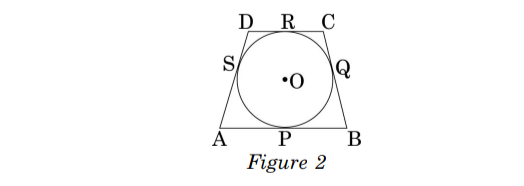
\includegraphics[width=0.8\textwidth]{q5.png} \\
    
\end{center}

\vspace{0.5cm}

\section*{Question 6}
\textbf{Prove that the points $(3, 0)$, $(6, 4)$ and $(-1, 3)$ are the vertices of a right-angled isosceles triangle.}
\begin{enumerate}
\setcounter{enumi}{6}
% You can continue adding more questions below...
\item The 4\textsuperscript{th} term of an A.P. is zero. Prove that the 25\textsuperscript{th} term of the A.P. is three times its 11\textsuperscript{th} term.
    
    \item Let P and Q be the points of trisection of the line segment joining the points A(2, -2) and B(-7, 4) such that P is nearer to A. Find the coordinates of P and Q.
    
    \item In Fig. 3, from an external point P, two tangents PT and PS are drawn to a circle with centre O and radius r. If OP = 2r, show that $\angle OTS = \angle OST = 30^\circ$.
    
    \begin{center}
        
\includegraphics[width=0.4\textwidth]{q9.png} % Replace with actual image if compiling
        \\
    \end{center}
    
    \item Solve for $x$: \quad $\sqrt{6x + 7} - (2x - 7) = 0$
\end{enumerate}

\section*{SECTION - C}
\textbf{Question numbers 11 to 20 carry 3 marks each.}

\begin{enumerate}
    \setcounter{enumi}{10}

    \item A conical vessel, with base radius 5 cm and height 24 cm, is full of water. This water is emptied into a cylindrical vessel of base radius 10 cm. Find the height to which the water will rise in the cylindrical vessel. (Use $\pi = \dfrac{22}{7}$)

    \item In fig. 4, O is the centre of a circle such that diameter AB = 13 cm and AC = 12 cm. BC is joined. Find the area of the shaded region. (Take $\pi = 3.14$)

    \begin{center}
        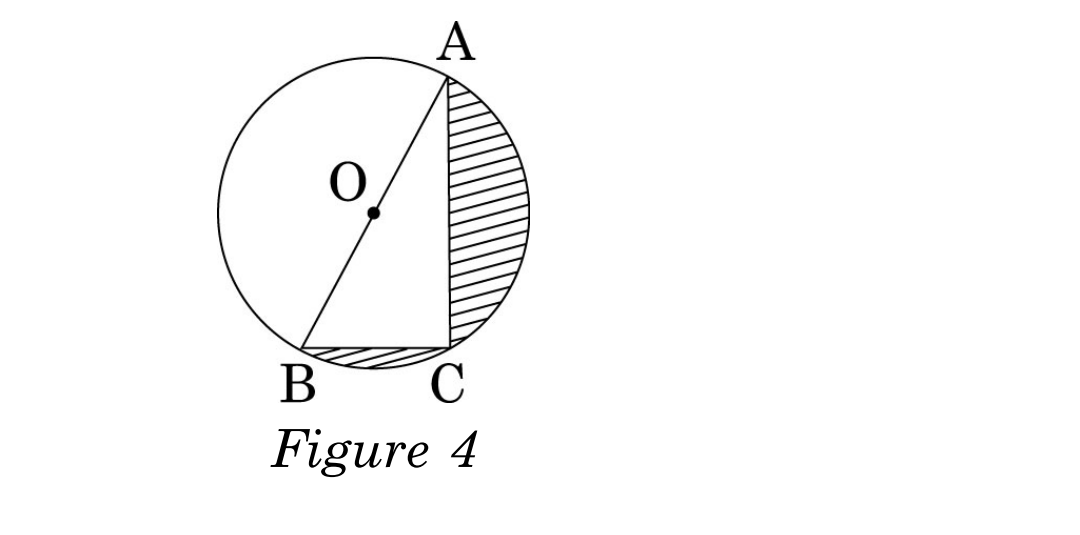
\includegraphics[width=0.7\textwidth]{p1.png
} % Replace with actual image path if compiling
        \\
    \end{center}

    \item If the point P(x, y) is equidistant from the points A(a + b, b - a) and B(a - b, a + b), prove that $bx = ay$.
\item If the point P(x, y) is equidistant from the points A(a + b, b - a) and B(a - b, a + b), prove that $bx = ay$.

    \item In fig. 5, a tent is in the shape of a cylinder surmounted by a conical top of same diameter. If the height and diameter of cylindrical part are 2.1 m and 3 m respectively and the slant height of conical part is 2.8 m, find the cost of canvas needed to make the tent if the canvas is available at the rate of 500/sq. metre. (Use $\pi = \dfrac{22}{7}$)

    \begin{center}
        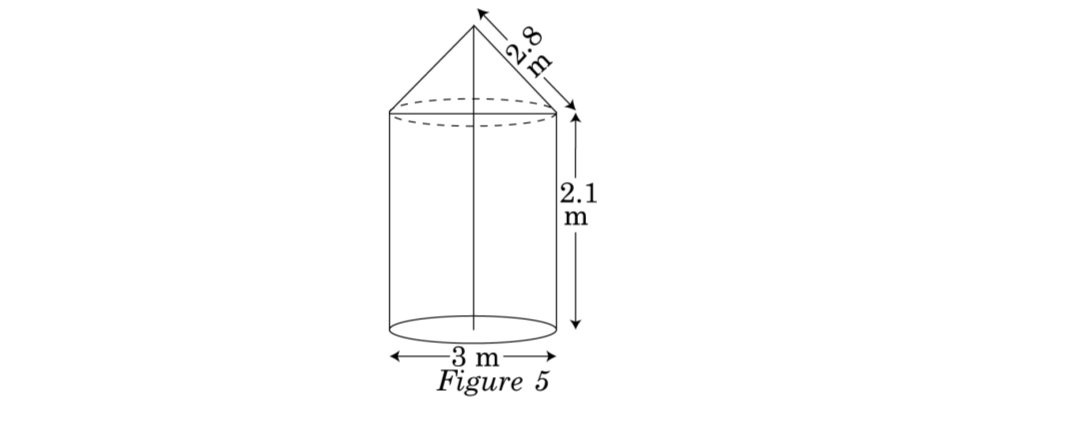
\includegraphics[width=0.9\textwidth]{l1.png} % Replace with actual image path
        \\
    \end{center}
\setcounter{enumi}{14}

    \item A sphere of diameter 12 cm, is dropped in a right circular cylindrical vessel, partly filled with water. If the sphere is completely submerged in water, the water level in the cylindrical vessel rises by $3\dfrac{5}{9}$ cm. Find the diameter of the cylindrical vessel.

    \item A man standing on the deck of a ship, which is 10 m above water level, observes the angle of elevation of the top of a hill as $60^\circ$ and the angle of depression of the base of hill as $30^\circ$. Find the distance of the hill from the ship and the height of the hill.

    \item In fig. 6, two concentric circles with radii 7 cm and 14 cm. Find the area of the shaded region between them, when $\angle AOC = 40^\circ$. (Use $\pi = \dfrac{22}{7}$)

    \begin{center}
        
\includegraphics[width=0.9\textwidth]{p2.png} % Replace with actual image path
        \\
\item{18} There are 100 cards in a bag on which numbers from 1 to 100 are written. A card is taken out from the bag at random. Find the probability that the number on the selected card\\
    (i) is divisible by 9 and is a perfect square\\
    (ii) is a prime number greater than 80.

    \item{19} Three consecutive natural numbers are such that the square of the middle number exceeds the difference of the squares of the other two by 60. Find the numbers.

    \item {20}The sums of first \(n\) terms of three arithmetic progressions are \(S_1\), \(S_2\) and \(S_3\) respectively. The first term of each A.P. is 1 and their common differences are 1, 2 and 3 respectively. Prove that \(S_1 + S_3 = 2S_2\).
    \end{center}
\end{enumerate}
\end{document}
